\documentclass[14pt,fleqn]{extarticle}
\usepackage[T2A,T1]{fontenc}
\usepackage[utf8]{inputenc}
\usepackage[russian]{babel}
\usepackage{amsmath}
\usepackage{graphicx}
\usepackage{tabularx}
\usepackage{boldline}
\usepackage{makecell}
\usepackage{arydshln}
\usepackage{mathtools}
\usepackage{centernot}
\usepackage{enumitem}
\usepackage{nccmath}
\usepackage{amssymb}
\usepackage[a4paper, total={6.5in, 9.5in}]{geometry}

\graphicspath{ {./images/} }
\setlength{\mathindent}{0pt}
\setlength\parindent{0pt}

\def\at{
	\left.
	\vphantom{\int}
	\right|
}


\begin{document}
	\begin{titlepage}
		
\includegraphics[scale=0.12]{logo}
		\begin{center}
			\textbf{МИНОБРНАУКИ РОССИИ}\\
			\vspace{0.2cm}
			\textbf{Федеральное государственное бюджетное образовательное учреждение высшего образования}\\
			\textbf{<<САНКТ-ПЕТЕРБУРГСКИЙ ГОСУДАРСТВЕННЫЙ ЭКОНОМИЧЕСКИЙ УНИВЕРСИТЕТ>>}\\
			\vspace{0.6cm}
			Факультет информатики и прикладной математики\\
			Кафедра прикладной математики и экономико-математических методов\\
			\vspace{1cm}
			\textbf{ОТЧЁТ}\\
			по дисциплине:\\
			\textbf{<<Модели экономической динамики>>}\\
			на тему:\\
			\textbf{<<Модель Солоу с человеческим капиталом. Задание №1>>}\\
		\end{center}
		\vspace{1cm}
		Направление: 01.03.02\\
		Обучающийся: Бронников Егор Игоревич\\
		Группа: ПМ-1901\\
		\vfill
		\begin{center}
			Санкт-Петербург\\
			2022\\
		\end{center}
	\end{titlepage}
    \subsection*{Задание}
    Составить модель Солоу с человеческим капиталом в относительных показателях. Выполнить качественный анализ модели.\\
    \newline
    
    \textit{Модель Солоу с человеческим капиталом:}\\

    $Y$ -- валовый внутренний продукт (ВВП)\\
    $K$ -- физический капитал\\
    $H$ -- человеческий капитал\\
    $L$ -- трудовые ресурсы\\
    $A$ -- технологический прогресс\\
    $s_K$ -- доля инвестиций на физический капитал\\
    $s_H$ -- доля инвестиций на человеческий капитал\\
    $\delta$ -- доля износа\\
    $n$ -- постоянный прирост трудовых ресурсов\\
    $g$ -- постоянный прирост технологического прогресса\\
    $\alpha$ -- эластичность выпуска по физическому капиталу\\
    $\beta$ -- эластичность выпуска по человеческому капиталу\\
    
    \begin{align*}
	& Y = K^{\alpha} \cdot H^{\beta} \cdot (AL)^{1-\alpha-\beta}\\
	& \dot{K} = s_K Y - \delta K\\
	& \dot{H} = s_H Y - \delta H\\
	& g_L = \dfrac{dL}{dt} = n\\
	& g_A = \dfrac{dA}{dt} = g\\
	& \alpha + \beta < 1\\
	\end{align*}

	\textit{Модель Солоу с человеческим капиталом в относительных показателях:}
    \begin{align*}
	& y = \dfrac{Y}{AL} \textup{ -- ВВП на душу населения с учётом технологического прогресса}\\
	& k = \dfrac{K}{AL} \textup{ -- фондовооружённость с учётом технологического прогресса}\\
	& h = \dfrac{H}{AL} \textup{ -- человековооружённость с учётом технологического прогресса}\\
	\end{align*}
	
	\newpage
	\begin{align*}
	& \dfrac{dk}{dt} = \left(\dfrac{K}{AL}\right)^{'} = \dfrac{\dot{K} AL - K(\dot{A}L + \dot{L}A)}{(AL)^2} = \dfrac{\dot{K}}{AL} - \dfrac{K}{AL} \cdot \dfrac{\dot{A}}{A} - \dfrac{K}{AL} \cdot \dfrac{\dot{L}}{L} =\\
	& = \dfrac{s_K Y - \delta K}{AL} - kg - kn = s_K \cdot y - (n + g + \delta) k
	\end{align*}

	\begin{align*}
	Y = AL \cdot k^\alpha \cdot h^\beta \quad \Rightarrow \quad y = k^\alpha \cdot h^\beta
	\end{align*}

	\begin{align*}
	& \dfrac{dh}{dt} = \left(\dfrac{H}{AL}\right)^{'} = \dfrac{\dot{H} AL - H(\dot{A}L + \dot{L}A)}{(AL)^2} = \dfrac{\dot{H}}{AL} - \dfrac{H}{AL} \cdot \dfrac{\dot{A}}{A} - \dfrac{H}{AL} \cdot \dfrac{\dot{L}}{L} =\\
	& = \dfrac{s_H Y - \delta H}{AL} - hg - hn = s_H \cdot y - (n + g + \delta) h
	\end{align*}
	\newline
	Итого:
	\begin{align*}
		& y = k^\alpha \cdot h^\beta\\
		& \dfrac{dk}{dt} = s_K \cdot y - (n + g + \delta) k\\
		& \dfrac{dh}{dt} = s_H \cdot y - (n + g + \delta) h\\
	\end{align*}

	\textit{Качественный анализ динамики:}\\
	
	Получается система из двух нелинейных дифференциальных уравнений:
	\begin{align*}
		\begin{cases}
		\dot{k} = s_K \cdot y_t - (n + g + \delta) k_t\\
		\dot{h} = s_H \cdot y_t - (n + g + \delta) h_t\\
		\end{cases}
	\end{align*}

	Как и в модели Солоу, каждое из уравнений имеет устойчивое состояние при нулевом спросе.
	\begin{align*}
		& \dot{k} = s_K \cdot y_t - (n + g + \delta) k_t = s_K \cdot k_t^\alpha \cdot h_t^\alpha - (n + g + \delta) k_t = 0\\
		& s_K \cdot k_t^\alpha \cdot h_t^\alpha = (n + g + \delta) k_t\\
		& k_t^{1-\alpha} = \dfrac{s_K \cdot h_t^\beta}{n + g + \delta}
	\end{align*}
	
	Преобразовав и выразив фондовооружённость, получим её значение при нулевом приросте фондовооружённости:
	\begin{ceqn}
	\begin{align*}
	 	k_t = \left[\dfrac{s_K}{n + g + \delta}\right]^{\frac{1}{1-\alpha}} h_t^{\frac{\beta}{1-\alpha}}
	\end{align*}
	\end{ceqn}
	\newpage
	Аналогично можно преобразовать второе дифференциальное уравнение:
	\begin{ceqn}
		\begin{align*}
			h_t = \left[\dfrac{s_H}{n + g + \delta}\right]^{\frac{1}{1-\beta}} k_t^{\frac{\alpha}{1-\beta}}
		\end{align*}
	\end{ceqn}
	
	Система уравнений локально устойчива, имеет действительные корни и тип равновесия будет -- <<устойчивый узел>>.
	
	\begin{figure}[h]
		\centering 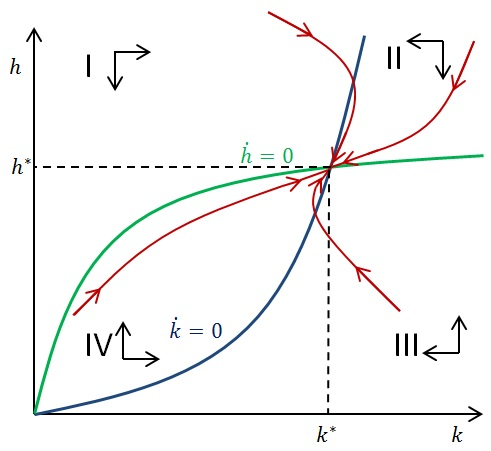
\includegraphics[scale=0.6]{plot_M-R-W}
		\caption{Фазовая диаграмма модели}
		\label{fig:plot_M-R-W}
	\end{figure}
	
	Устойчивое состояние модели можно выразить, подставляя полученные уравнения одно в другое:
	\begin{ceqn}
		\begin{align*}
			k^* = \left(\dfrac{s_K^{1-\beta} \cdot s_H^\beta}{n + g + \delta}\right)^{\frac{1}{1-\alpha-\beta}}\\
			h^* = \left(\dfrac{s_K^{1-\alpha} \cdot s_H^\alpha}{n + g + \delta}\right)^{\frac{1}{1-\alpha-\beta}}
		\end{align*}
	\end{ceqn}

	\begin{ceqn}
		\begin{align*}
			y^* = \left(\dfrac{s_K^{\alpha} \cdot s_H^\beta}{(n + g + \delta)^{\alpha+\beta}}\right)^{\frac{1}{1-\alpha-\beta}}\\
		\end{align*}
	\end{ceqn}
	
	Линии $\dot{k} = 0$ -- синяя и $\dot{h} = 0$ -- зелёная делят диаграмму на четыре квадранта. Возможные траектории фондовооружённости показаны красным. В итоге, в модели из любой начальной точки система приходит к равновесию ($k^*, h^*$).
\end{document}
